% Generated by scripts/export_qsart_x_tables.py. Compile from the repository root with graphicx.
% Set-C evaluation SHA-256: 14c7ed44bfec0f66ac8a5763ca093f9a70c599438fb545368918f47dc0d4069a
% Paired-view evaluation SHA-256: 230c5bab0851c2ee708e3d52f5fd066bc383dcfd6168d1c0f01b14ca07becd48

\begin{table*}[t]
\centering
\caption{Deployed ordinal dual-budget policy on DeepDRiD Set-C (99 patients).}
\label{tab:qsart-set-c}
\begin{tabular}{llrr}
\hline
Image caps & Status & Review & Automatic \\
\hline
30\% / 20\% & Overload & -- & -- \\
60\% / 40\% & Overload & -- & -- \\
90\% / 40\% & Overload & -- & -- \\
100\% / 40\% & Evaluated & 99 & 0 \\
\hline
\end{tabular}
\end{table*}

\begin{table*}[t]
\centering
\caption{Retrospective paired-view acquisition on 84 eyes. Misses count eye-level missed referrals.}
\label{tab:qsart-paired-views}
\begin{tabular}{lrrrr}
\hline
Policy & Views & Misses & Severe & Cost/eye \\
\hline
First view only & 0 & 8 & 4 & 0.5833 \\
Estimated-value ranking & 8 & 6 & 3 & 0.4536 \\
Estimated value above cost & 4 & 8 & 4 & 0.5929 \\
Estimated-value ranking & 21 & 6 & 3 & 0.4875 \\
Estimated-value ranking & 42 & 6 & 3 & 0.5375 \\
Estimated-value ranking & 63 & 6 & 3 & 0.5875 \\
Both recorded views & 84 & 6 & 3 & 0.6286 \\
\hline
\end{tabular}
\end{table*}

\begin{figure*}[t]
\centering
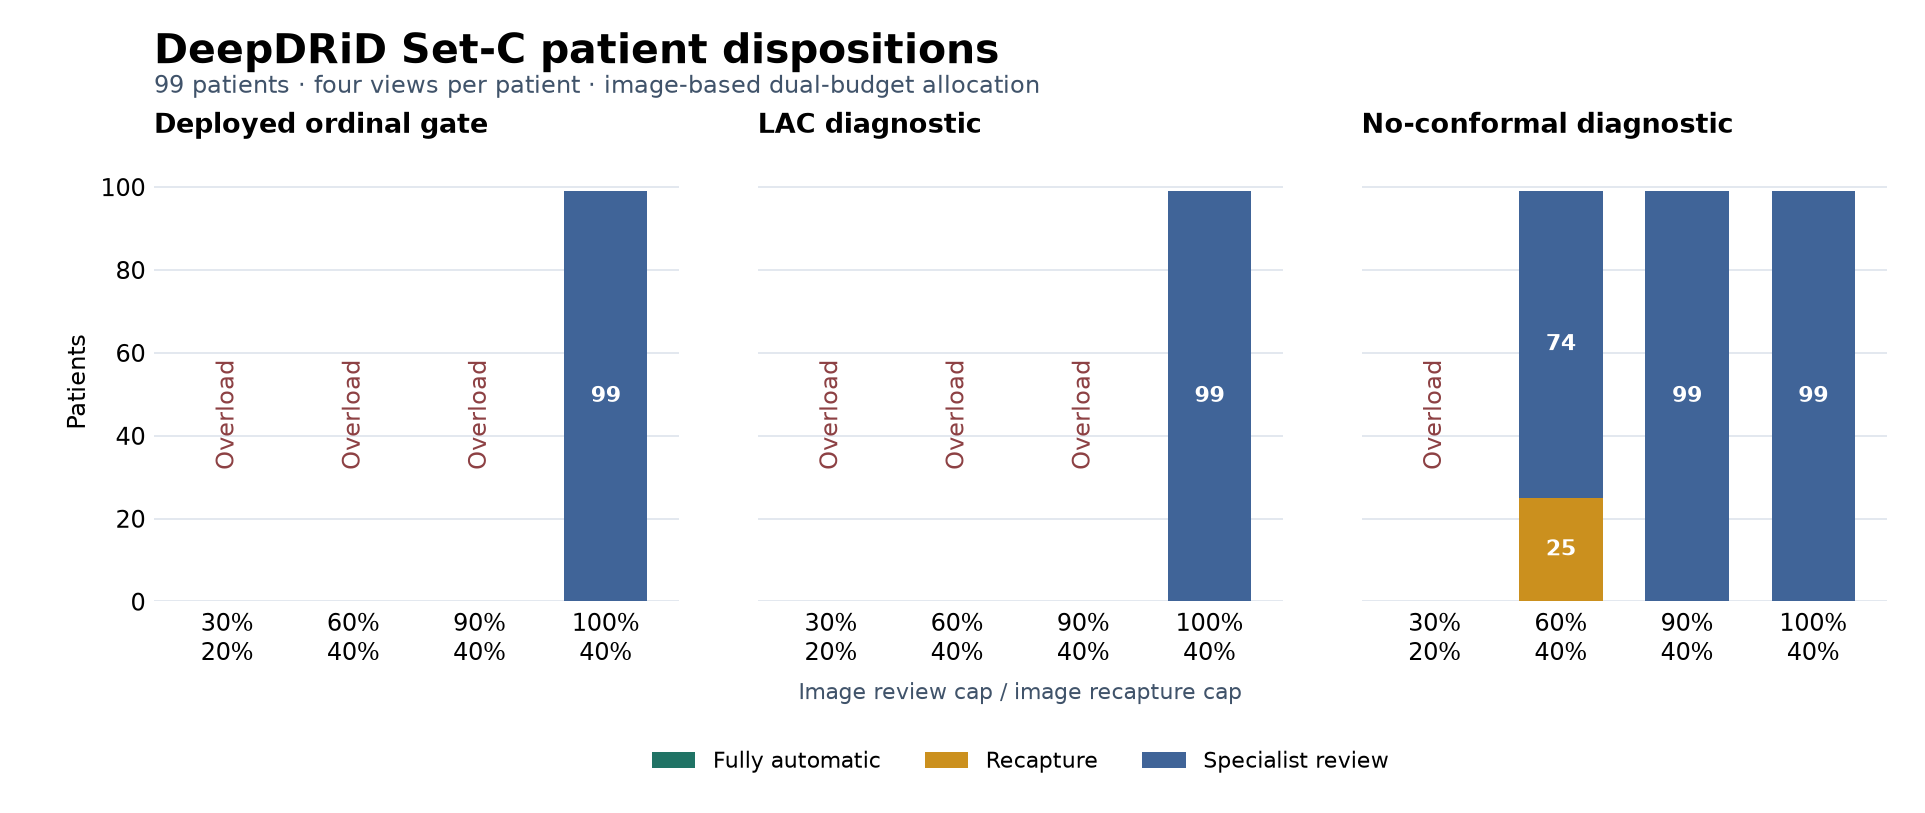
\includegraphics[width=\textwidth]{reports/set_c_validation_v1/patient_dispositions.png}
\caption{Patient recommendations under the deployed ordinal gate and two diagnostic variants.}
\label{fig:qsart-set-c}
\end{figure*}

\begin{figure*}[t]
\centering
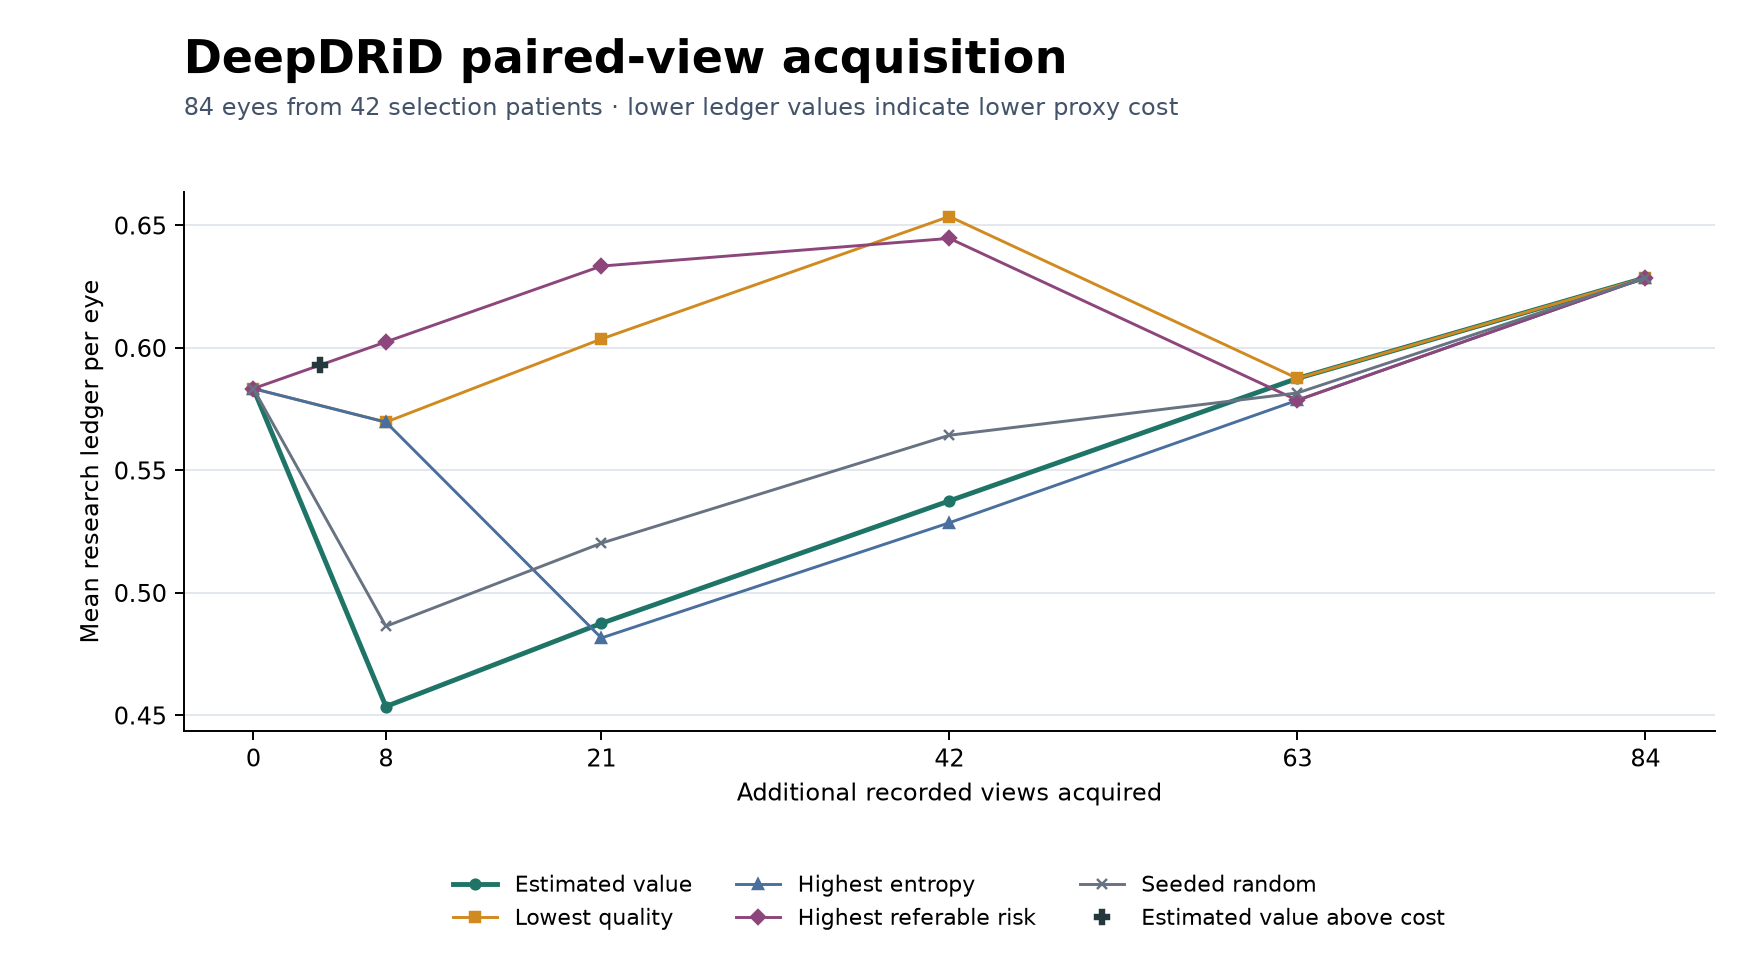
\includegraphics[width=\textwidth]{reports/paired_view_v1/acquisition_workload.png}
\caption{Research ledger by the number of additional recorded views.}
\label{fig:qsart-paired-views}
\end{figure*}
